%!TEX root = main.tex
\chapter{Introduction}
  \label{ch:intro}
  \begin{quotation}
    \small
    \textit{``It is now plain that about 75\% of the data we would like to have can be obtained from good ground-based sites''}

    -H. Johnson, 1966
  \end{quotation}

\section{All-sky Astronomy}
    All-sky astronomy is not new. Indeed, the notion of capturing a particular ``object'' or ``source'' with a camera and saving it for later investigation would be completely alien to the first astronomers and astronavigators. Absence of telescopes forced us to describe the sky in terms of its larger patterns, brightest characters. What is new however is the notion of preparing an archive of the sky itself for not only the research whims of a single investigator, team, institute, or even a single nation\- rather, all-sky surveys tend to be international endeavors in their production, and even more so in their utilization.
      \begin{table}
        \renewcommand\arraystretch{1.4}
        \captionsetup{singlelinecheck=false, labelfont=sc, labelsep=quad}
        \caption{Timeline of all-sky surveys}\vskip -1.5ex
          \begin{tabular}{@{\,}r <{\hskip 2pt} !{\foo} >{\raggedright\arraybackslash}p{5cm}r}
            \toprule
            \addlinespace[1.5ex]
            1983 & IRAS    & \cite{iras84} \\
            1989 & COBE    & \cite{boggess92}\\
            1990 & ROSAT   & \cite{truemper82}\\
            2001 & WMAP    & \cite{wmap03a}\\
            2003 & 2MASS   & \cite{skrutskie06}\\
            2003 & GALEX   & \cite{martin05} \\
            2006 & AKARI   & \cite{akari07} \\
            2008 & Fermi   & \cite{atwood09} \\
            2009 & Planck  & \cite{planckEarly11I}\\
            2009 & WISE    & \cite{wright10} \\
          \end{tabular}
      \end{table}


  \section{Infrared astronomy}

    Infrared astronomy was essentially non-existant as recently as the 1920s, if we judge by the first IR observations \citep{pettit22, pettit28}. Mainstream IR astronomy is perhaps much younger, only really taking off --- literally --- in the post-war era, via ballon and rocket borne experiments \citep{johnson66}. Compare this to visible wavelengths, a field so old we name it after the bio-evolutionary advent of sight, itself. Even radio astronomy with its own logistical and technological challenges, has been around since at least 1932.

    Astronomers have not been content to be constrained by atmospheric IR windows, even from the best of ground-based sites. Or perhaps interests have shifted so dramtically since 1966, that all of the investigations enabled by rocket-based, space-based, even Boeing 747-based IR astronomy (e.g. SOFIA, the Stratospheric Observatory for Inrared Astornomy,\cite{young12}) would have bored 75\% of astronomers in the '60s. The meaning of ``far infrared'' has even redshifted, so to speak, from the \cite{johnson66} definition of ``4 to 22~$\mu$m'' --- consider the ``Far Infrared Surveyor'' instrument onboard the AKARI satellite \citep{akari07}, which observed from 50 to 180~$\mu$m \citep{kawada07}

     For our purposes, we consider the FIR to cover 60 to 550~$\mu$m, partially out of convenience- FIR bands, in this paper, means the Infrared Astronomical Satellite (IRAS) 60 and 100~$\mu$m \citep{iras84}, all four FIS bands, and the Planck Observatory's High Frequency Instrument (HFI)~857~GHz and 545~GHz bands \citep{planckEarly11I, hfi14viii}. The two AKARI Infrared Camera (IRC) \citep{irc07,ishihara10} bands and the IRAS~12 and 25~$\mu$m bands we will refer to collectively as the mid-infrared (MIR) bands.

 \section{Multi-wavelength investigations}

     The ability to map and archive the sky with satellites -- not only in the optical and infrared, but well into the microwave regime -- has enabled interdisciplinary research of the interstellar-medium (ISM). The ISM pervades the galaxy and either surrounds or intervenes basically any object one may wish to study. The ISM is enriched as matter is processed and flows back into space. We can describe the ISM as a mixture of gas and dust. An early estimate by \cite{knapp74} puts the mass of dust in the galaxy at about 1\% that of interstellar gas.

    A wealth of data is now available not only in the IR, but on into the sub-millimeter range and the interpretation of this data has become a serious priority. This is especially true for the last ten years as new, much higher resolution surveys have been carried out such as the Spitzer Space Telescope \cite{spitzer04}, Herschel Space Observatory (Herschel) \citep{herschel10} by NASA and the ESA respectively, and the AKARI telescope \citep{akari07},  by JAXA. AKARI especially, produced a wealth of data spanning the entire sky. It was equipped with IRC \citep{irc07} to study the MIR, and FIS \citep{fis07} to study cooler dust and gas, and conduct spectroscopy in the far infrared (FIR) via its built-in Fourier Transform Spectrometer (FTS). The FIS all-sky maps have just been publicly released at the time of this writing (Doi, et al. 2014). The IRC all-sky maps are soon to follow. In this thesis we use these AKARI surveys in a comparison with other cutting edge all-sky maps from the Planck Observatory in a multi-wavelength study of yet another part of the ISM puzzle, the AME and its connection to interstellar dust.
    
    The merits of multiwavelength based investigations arise from the simple fact that the ISM is very complex--- both in terms of the myriad forms of matter present, from plasmas to dust grains --- and in countless physical processes at play. Consider the complex case of a supernova remnant influencing surrounding ISM: through a combined analysis of radio, mid-far infrared, and X-ray data, \cite{lau15} were able to characterize the history of dust production, heating, and destruction within the Sgr A East supernova remnant.


\section{Interstellar Dust}

    The study of interstellar dust has been connected to mainstream astrophysics research, and recognized as an integral player in the evolution of the interstellar medium. This has been shown by early sounding rocket experiments \citep{wolstencroft67,soifer71}, and balloon experiments \citep{muehlner70,emerson73}, and dust has been more profoundly exposed by the advent of all-sky infrared surveys like the  Cosmic Microwave Background Explorer's Diffuse Infrared Background Experiment (COBE/DIRBE) \citep{sodroski94} and the Infrared Astronomical Satellite (IRAS) \citep{iras84}.
    With space-borne long-term IR mapping finally available on an all-sky scale, we could move past the interplanetary medium and into the interstellar.

  The role of dust in the interstellar medium has expanded beyond simply an intervening, stellar light obstructing material. Theoretical models and observations have shown that dust grains act as a catalyst for the formation of molecular hydrogen and other molecules, providing a substrate upon which hydrogen and other atoms can meet \citep{iglesias77,burke83}. With infrared observations we are able to study dust directly via its vibrational emission, rather than relying only on inference from visible reddening and polarization effects \citep{davis51,platt56, carrasco73}.
   The question of the composition of dust has grown from a single thread of investigation into a network of questions. Many pieces in this dusty puzzle are missing. For example, the presence of dust grains containing silicates, and amorphous carbon is very strongly supported by comparisons of infrared spectroscopy with laboratory studies \citep{hagen79,joblin09}. But many questions remain about which silicate and carbonaceous species may be present, and in what proportions, and in what distribution of sizes. The question also remains, is there more to dust than simply carbonaceous and silicate grains?  The exact size distribution of dust grains is also an open question. The composition of extremely small grains / large molecules is a particularly challenging mystery, as well as the role of interstellar ices in the evolution dust and gas.

\subsection{Silicate grains}
     One of the first materials proposed to exist as interstellar dust were silicates, with the first evidence being UV absorption features \citep{knacke69}. More recently, specific species of silicates are being identified via absorption spectroscopy \citep{olofsson12}. However some doubt has been cast recently on the structure of the grains. For example, in \cite{jones13} and \cite{jones14} an updated model is proposed wherein dust grains may be composed of a mixture of silicate and amorphous carbon material, such as a silicate core with an amorphous carbon envelope, representing the first comprehensive model of continuous grain evolution. In other words, the first model to consider dust grain morphology beyond the descrete categories of silicate grains, carbonaceous grains, and polycyclic aromatic hydrocarbons (PAHs). An additional feature of this model is that silicates having iron inclusions are expected, which would be similar to the Fe form of olivine. This is an update from the conventional ``astronomical  silicates" assumed in earlier dust spectral energy distribution (SED) models such as \cite{li01} or \cite{dustem11}.

\subsection{Carbonaceous grains}
      As with silicates, the existance well-established that carbonaceous material, primarily amorphous carbon, exists in the ISM \citep{aitken81,tielens87}. This is material commonly called ``soot" or the fuel we know on earth as coal.    Some non-amorphous carbonaceous material is also speculated to exist, such as graphite \citep{zhou06} or ``buckyonions" (concentric-shell-graphite) \citep{li08}.

\subsection{Size distribution of dust grains}

\subsection{Polycyclic Aromatic Hydrocarbons and the Unidentified Infrared Bands}

    From the mid-to-near IR however, spectroscopic observations enabled and required the simple two-populations model of larger and smaller dust (e.g. \cite{mathis77}), to be expanded. ``Unidentified IR bands'' from~ 3 to 11~$\mu$m (hereafter, UIR bands), demonstrate another divergence from the canonical dust emission story. The UIR bands were first reported at 8 to 13~$\mu$m in planetary nebulae and HII regions by \cite{gillet73, gillett75} in ground-based observations. Observations by \cite{merrill75} noted another unexplained feature at 3.27~$\mu$m, noting: ``there are [...] similarities in the 8-13~$\mu$m spectra of NGC 253, NGC 7027, and BD +30$^\circ$3639 \cite{gillett75}''. Features at 6.2 and 7.7~$\mu$m were reported by \cite{russell77b} using the first airplane-mounted IR telescope and predecessor to SOFIA, the Kuiper Airborne Observatory. \cite{sellgren83} reported features at 3.3 and 3.4~$\mu$m being detected in reflection nebulae.

     Within  the last 30 years, a popular hypothesis has arisen that a particular set of features of the interstellar medium SED between 3 and 12 microns, known as the ``Unidentified Infrared Bands" (UIRs), can be explained by the PAH family of molecules. The PAH interpretation was first proposed by \cite{allamandola85} and \cite{puget85}.
     With the appearance of high powered computers with an ability to perform rigorous calculations, many attempts have been made to simulate the expected emission from PAHs. Density functional theory (DFT) \citep{honenberg64} has become available as a tool for simulating molecular emission features using a quantum approach. DFT calculations has become a subfield of ISM astrophysics. Many attempts are being made to fit particular emission features of PAHs, and other molecular and grain species, to observed ISM features \citep{hammonds09,hirata99}.
     While it is difficult to reproduce the exact interstellar conditions in a laboratory setting, DFT simulations have yielded some evidence that the UIR bands can be explained as PAH vibrational emission features \citep{pathak12,ricca11,yu12}.

    We should note however that PAHs are not the only proposed explanation for the UIR features, despite being the most widely accepted. \cite{zhang14} propsed theoretically that mixtures of non-PAH carbonaceous and silicate spectra could also fit theoretically calculated PAH emission features. However the PAH-UIR hypothesis is still widely supported \citep{tielens08,rastogi13}. The way that PAHs might be produced or evolve from other species is not understood however. Though there are efforts underway to model potential formation pathways. As far as the evolution of larger aromatics form smaller PAHs, there is one proposed pathway wherein a benzene could grow into a larger aromatic molecule such as naphthalene \citep{ghesquiere14}.

     From this point, the UIR bands become much less of property of select objects in targeted observations, are seen observed throughout the Milky Way. Balloon-based observation by \cite{giard94} confirmed that the 3.3~$\mu$m feature pervades throughout the Galactic plane. The first-ever airborne IR observatory, Kuiper Several years later, space-based spectroscopy with the Infrared Telescope in Space (IRTS)\citep{murakami96} and Infrared Space Observatory (ISO)\citep{kessler96} enabled confirmation by \cite{onaka96} and \cite{mattila96} that the mid-infrared UIR features are not limited to selection objects, but are present even in the diffuse galactic ISM by. \cite{dwek97} even reported that photometric excess in the COBE/DIRBE 12~$\mu$m band may be caused by the UIR bands, in and suggested they may be from these UIR features have come to be explained via polycyclic aromatic hydrocarbons (PAHs), a possibility which had been considered earlier by \cite{allamandola85,puget85}. PAHs are a class of molecules composed primarily of fused carbon rings such as corranulene. PAHs and/or similar amalgems containing aromatic structures (e.g. quenched carbonaceous composites (QCCs), \cite{sakata84}) have been incorporated into dust mixture SED models over the last two decades \citep{drli01, drli07, hony01, dustem11, galliano11, jones13, jones17}.

    Moving in the opposite direction, into the Rayleigh-Jeans regime of thermal dust emission, multi-wavelength observations have opened up a new discipline: the disentagnlement of interstellar dust emission from non-dust emission components. Most notably, separating fluctuations in the cosmic microwave background (CMB) from the microwave extent of thermal dust emission. Those studying the Milky Way itself, from the far IR into microwave and radio frequencies, are now collaborating closely with those interested in the precise nature of the CMB.

\section{Microwave foregrounds}

    Much of the motivation between recent galactic microwave emission research has little to do with galactic ISM astronomy itself. Rather, our galaxy presents an inconvenience to observational cosmology in that it 'contaminates' observations of the CMB. The avereage SED of the CMB is simple enough to model, with a 2.755~K blackbody function. This temperature however means that the peak occurs between several microwave foreground components, from interstellar dust and gas, as displayed in Fig.~\ref{fig:mw_foregrounds_demo_rOph}. The difficulty of decomposing the microwave sky into galactic ISM, extragalactic, and CMB components has brought the detailed decomposition of the microwave\-radio regime of ISM to the forefront of Planck Collaboration paper titles \citep{planckEarly11I,planck2013I,planck2015I}. Without extragalactic research, there would be no need for the word ``foreground'' in describing galactic microwave emission.

    The ISM has intruded into cosmological studies perhaps most prominently with the first claimed detection of B-mode polarization \citep{hanson13, bicep214, flauger14}, and multiple response papers. The main consensus being that the validation of CMB-related claims require a careful estimate of the contribution, in intensity and polarization, from interstellar dust and the subsequent counter\-claim that this detection arose from galactic dust\citep{planckIntL17, sheehy17}. More recently \cite{shimwell12} had noted a peculiar Sunyaev\-Zeldovich effect based galaxy cluster detection, AMI-CL~J0300+2613. \cite{perrott18} have since proposed that this may in fact arise from high galactic latitude dust via ``anomalous microwave emission'' (AME).

  \subsection{Anomalous Microwave Emission}
      In our efforts to decompose and understand galactic microwave emission itself, there remains a constant antagonist. Galactic foregrounds had been broken down into 3 dominant components: free-free emission from ionized regions, synchrotron emission generated by electrons relativistically by the Milky Way's magnetic field, and the microwave extent of thermal dust emission \citep{wmap03b, leach08, planckXII}. Deviations from this understanding began to appear in the early 1990s, with efforts by \cite{kogut96, leitch97} to carefully investigate the CMB. They had found a component of the microwave sky which implied unlikely spectral indices for free-free or synchrotron emission. AME generally takes the form of an 'excess' continnuum emission source, having a peak somewhere between 10 to 40~GHz (see Fig.~\ref{fig:mw_foregrounds_demo_rOph}).
            \begin{figure}
              \centering
              \includegraphics[width=\textwidth]{../Plots/ch_intro/mw_foregrounds_demo_rOph.pdf}
                \caption{An example of a potential makueup of microwave emission components. Photometry points are extracted from the Planck and WMAP all-sky maps \citep{hfi14viii}, for a part of the region well-known for prominant AME, $\rho$~Ophiuchus \citep{planckxx11}. The AME curve is produced from a warm neutral medium spinning dust template \citep{ali-haimoud09}, with a frequency-shift applied to approximately fit the microwave data s in \cite{planck15X}}
              \label{fig:mw_foregrounds_demo_rOph}
            \end{figure}
        This excess defies predictions for known microwave emission mechansisms. AME still lacks a concrete physical explanation. Also, the term itself can be a bit confusing, as the word ``anomalous'' tends to imply localized outlier. The AME is shown to be more than an isolated anomaly, but an added component of microwave emission appearing throughout the galaxy \citep{deoliveiracosta97,wmap03b,dickinson13r}. Fig~\ref{fig:AME_contours} shows two prominent AME regions, $\rho{}$~Ophiuchus and the Persues Molecular Cloud investigated by \cite{tibbs11,planckxx11}, as they appear in AKARI/IRC~9$\mu$m all-sky map \citep{ishihara10}.
            \begin{figure}
              \centering
              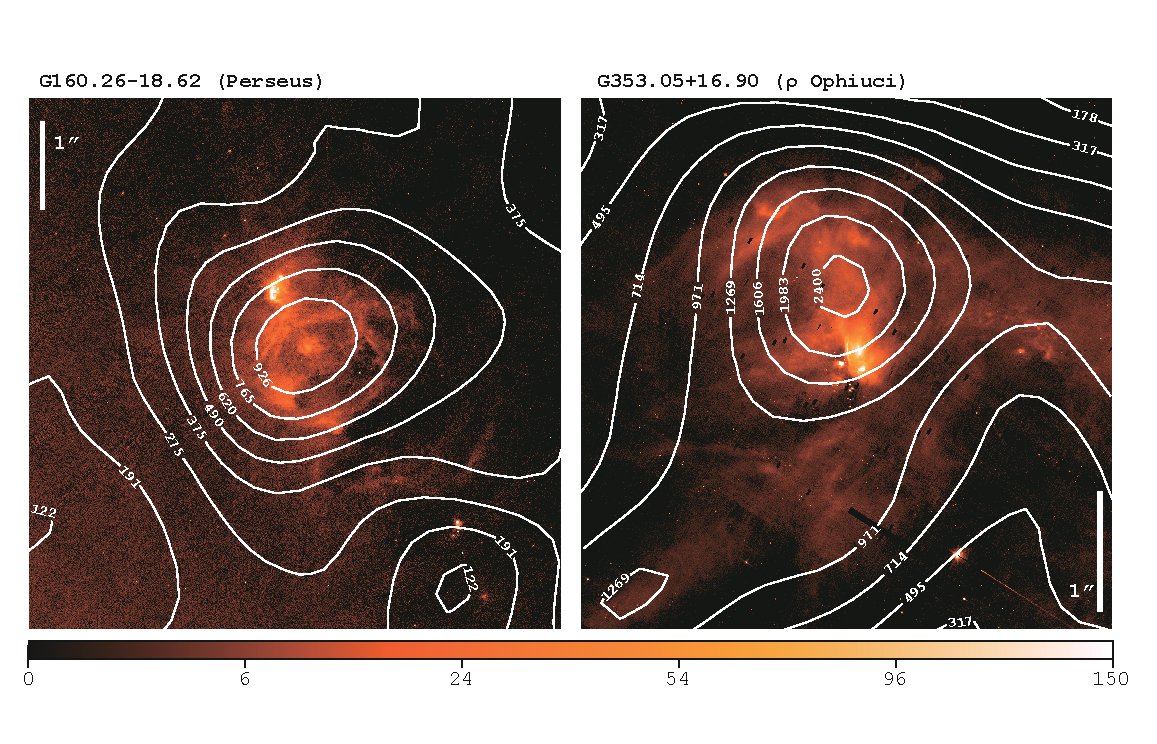
\includegraphics[width=\textwidth]{../Plots/ch_intro/AME_contours.pdf}
                \caption{Two AME prominent regions investigated by \cite{planckxx11, tibbs11}, $\rho$~Ophiuchus and Perseus, as they appear in the PAH-feature-tracing AKARI/IRC 9$\mu$m all-sky data at native resolution \citep{ishihara10}. White contours show AME at 1-degree resolution, extracted from the map by  \cite{planck15X}. The IRC data shown here is of a much finer resolution than the AME data, at around 10'', demonstrating the critical gap in resolvability of all-sky AME-tracing data itself vs. the IR dust tracers we hope to compare it to. }
              \label{fig:AME_contours}
            \end{figure}
        In this section we will explain that while there is indeed much mystery as to the exact mechanism(s) producing the AME, what causes its spectral variations, and what might be its physical carrier(s) - it is by now, perhaps less than anomalous. Following subsections will discuss the history of AME and the produced physical explanations, as well comparisons between the AME and infarred emission from interstellar dust.

    \subsubsection{Correlation with dust}
         Since its first detection in early microwave observations, AME has been found to be a widespread feature of the microwave Milky Way (see the review \cite{dickinson13r}, and an updated state-of-play of AME research by Dickinson et al. (in prep). \cite{kogut96,deoliveiracosta97} showed that the AME correlates very well with infrared emission from dust, via COBE/DIRBE and IRAS far-IR maps.  \cite{finkbeiner02} reported the first detection of a ``rising spectrum source at 8~to~10~GHz'' in an observation targeting galactic ISM cloud. \cite{deoliveiracosta02} furher argued that this emission is in fact ``ubiquitous''. The exact mechanism and carrier/s remain mysterious however.
        More recent works, employing observations by the Wilkinson Micrwave Anisotropy Probe (WMAP), Spitzer Space Telescope, the latest IR to microwave all-sky maps by Planck, and various ground based radio observations have strongly confirmed a relationship between interstellar dust emission and AME \citep{ysard10a,tibbs11,hensley16}. Exactly which physical mechanisms produces the AME however is still an open question, even if we assume a dusty AME origin. We equally puzzled as to the chemical composition and morphology of the carrier(s). We also lack an all-sky constraint on the emissivity of the AME spectrum at frequencies short of the WMAP cut-off, around 23~GHz. The typical peak frequency of AME, in those cases where it is constrained, does give us a clue.

  \subsection{Proposed explanations}
     From the observed spatial correlation between AME and dust emerged two prevailing hypotheses:

    1) Electric dipole emission by spinning small dust grains, a mechanism proposed in \cite{erickson57} and \cite{hoyle70}, with further discussion in \cite{ferrara94}. \cite{draine98b} give the earliest thorough theoretical prediction of a spinning dust spectrum. A decade later \cite{ali-haimoud09} contributed substantial updates, expanded modeling of grain excitation mechanisms and adoption of an updated grain size distribution by \cite{weingartner01}. \cite{ysard10a} introduced the first model of a spinning dust spectrum based on rotational emission from polycyclic aromatic hydrocarbons (PAHs), which are implicated due to their size.  \cite{draine98b}, gives the expected rotational frequency of spinning dust oscillators $\omega$,  as follows:
        \begin{equation}
        {\omega_T\over 2\pi} =
        \langle\nu^2\rangle^{1/2}
        \approx 5.60\times 10^9 a_{-7}^{-5/2}\xi^{-1/2}T_2^{1/2}~~~{\rm Hz},
        \label{eq:nurms}
        \end{equation}
    where $T$ is the gas temperature, $a$ is the grain size, and $\xi$ represents the deviation from a spherical moment of intertia. For example, we can take a typical peak frequency of the AME of \textasciitilde{}20~GHz, a gas temperature of 100~K, roughly spherical grains, and a dipole moment on the order of 1~debye, and get:
        \begin{equation}
            {\omega_T\over 2\pi} =
                20~GHz({T\over 100K})^{1/2}({\rho \over{3gcm^{03}}})^{-1/2}({a\over 5\AA{}})^{-5/2}
            \label{eq:nurms_ex}
        \end{equation}
    implying an oscillator size of approximately 1~nm. Thus PAHs, as considered by \cite{ysard10a}, are a primary candidate spinning dust carrier, due to their expected size range.

    2) Magnetic dipole emission, caused by thermal fluctuations in grains with magnetic inclusions, proposed by \cite{draine99}.
     More recently, modeled spectra for potential candidate carriers have appeared in the literature: PAHs, grains with magnetic inclusions \citep{draine13, ali-haimoud14, hoang16a}.

    A third, but not widely accepted, possible explanation for AME is discussed in \cite{jones09}. They have suggested that the emissivity of dust, in the spectral range related to AME, could contain features caused by low temperature solid-state structural transitions.

    \subsubsection{Spinning dust}
     Spinning dust need not be the only emission mechanism, a convention as arisen in AME observational works. The photometric signature of the AME is frequently interepreted via spinning dust parameters \citep{ysard11,ali-haimoud10}. Archival all-sky AME data products exclusively assume a spinning dust SED templates. Both WMAP and Planck used a base template with 30~GHz peak frequency, and an assumed cold neutral medium evironment. Using the ``spdust'' spinning dust SED model code to fit excess microwave foreground emission has become analagous fitting a modified blackbody function to the far IR.

      We explore the case that the AME signature arises from spinning dust emission. If the AME is carried by spinning dust, the carrier should be small enough that it can be rotationally excited to frequencies in the range of 10-40~GHz, and must have a permanent electric dipole. Within contemporary dust SED models, only the polycyclic aromatic hydrocarbon family of molecules (PAHs), or nanoscale amorphous carbon dust fit these criteria. Those PAHs which have a permanent electric dipole (i.e. coranulene, but not symmetric molecules like coronene), can emit rotationally. However the carrier need not be carbon-based. Indeed, \cite{hensley17a} claim that AME can be explained without carbonaceous carriers, using only spinning nanosilicates.

     \subsubsection{Spinning PAHs?}
       Assuming the rotational emission model of \cite{draine98b}, the AME signature (consistent with peaked, continuum emission having a peak between 15 and 50~GHz ) implies very small oscillators (\textasciitilde{}1~nm).

       In any case, the PAH class of molecules are the only spinning dust candidate so far which show both: \\
       1) Evidence of abundance in the ISM at IR wavelengths, and \\
       2) A predicted range of dipole moments (on order of 1~debye), to produce the observed AME signature \citep{draine98b, lovas05, thorwirth07}.

       However, it should be noted that although nanosilicates have not yet been detected in the ISM, \cite{hensley17a} propose that an upper bound on the abundance of nanosilicates by \cite{li01} (based on IRTS observations by \cite{onaka96}), allow such small spinning grains to be composed primarily of silicates.

    While neither nanosilicates nor any particular species of PAHs have been conclusively identified in the ISM, there is far more empiracal evidence for PAH-like dust than for nanosilicates. Mid-infrared features associated with PAH-like aromatic materials have been observed. In fact, ``the PAH features'' are ubiquitous in the ISM \citep{giard94,onaka96,onaka00}, such that the carriers must be abundant. \cite{andrews15} strongly argue for the  existence of a dominant ``grandPAH'' class, containing 20 to 30 PAH species.

     \subsection{Excitation factors}
       In the spinning dust model, there are several possible excitation factors for spinning dust. For the grains to have rotational velocities high enough to create the observed AME, they must be subject to strong excitation mechansisms. The dominant factors that would be giving grains their spin, are broken down by \cite{draine11} into basically two categories: 1) Collisional excitation. 2) Radiative excitation, the sum of which could lead to sufficient rotational velocities for sufficiently small grains. However the extent of excitation will depend on environmental conditions, i.e. there will be more frequent encounters with ions and atoms in denser regions (so long as the density is not high enough to coagulate the small grains), and more excitation due to photon emission with increasing ISRF strength \citep{ali-haimoud09, ali-haimoud14}. One of the strongest potential excitation mechansims listed in \cite{draine11} is that of negatively charged grains interacting with ions. Thus not only must we consider environmental factors, grain composition and size, but also the ionization state of the carriers. (For example, ionized vs. neutral PAHs.) The dependence of the observed AME on ISM density is modeled by \cite{ali-haimoud10}.

       \subsection{AME vs. IR in the literature}
          The overall pattern among large-scale studies seems to show that all of the dust-tracing photometric bands correlate with the AME (and each other) to first-order.  On an all-sky, pixel-by-pixel basis, at 1$^{\circ}$ angular resolution, \cite{ysard10b} find that 12~$\mu$m emission, via IRAS, correlates slightly more strongly with AME (via WMAP) than with 100~$\mu$m emission.  They also find that scaling the IR intensity by the interstellar radiation field strength (given as $U$, a measure of ISRF relative to that of the solar neighborhood) improves both correlations. They interpret this finding as evidence that AME is related to dust, and more closely related to the small stochastically emitting dust --- predominantly PAHs --- that is traced by 12~$\mu$m emission. The improvement of the correlations after scaling by $U$ is expected, as long as the 12~$\mu$m or 9~$\mu$m photometric bands are by stochastic emisson from PAHs, in other words:
          \begin{equation}
            I_{12~\mu{}m} \propto{} UN_{PAH},
          \end{equation}
          where $N_{PAH}$ is the column density of emitting PAHs \citep{onaka00}. Thus it implies that $I_{12~\mu{}m}/U$ is giving us a measure of the column density of spinning dust.

          In a similar work however \cite{hensley16} report a lack of support for the spinning PAH hypothesis. Finding that fluctuations in the ratio of PAH-dominated 12~$\mu$m emission (via WISE) to dust radiance, $R$, (via Planck) do not correlate with the ratio of AME intensity to $R$, they conclude that the AME is not likely to come from PAHs. In terms of emission intensity however, their findings are consistent with \cite{ysard10b} in that $I_{12~\mu{}m}$ correlates well with $I_{AME}$. Thus there remains an open question as to what the actual carrier of the AME is.

         The story is no more clear when looking at the average properties of individual regions. \cite{planckXV} find that among 22 high-confidence ``AME regions'' (galactic clouds such as the $\rho$~Ophiuchus cloud and the Perseus molecular cloud complex) AME vs. 12~$\mu$m  shows a marginally weaker correlation than AME vs. 100~$\mu$m (via IRAS). \cite{tibbs11} examined the AME-prominent Perseus Molecular Cloud complex, finding that while there is no clear evidence of a PAH-AME correlation, they do find a slight correlation between AME and $U$.

\section{Statistical Methods}

  \subsection{Correlation tests}
     \begin{equation}
     \rho_{X,Y}= \frac{\operatorname{cov}(X,Y)}{\sigma_X \sigma_Y}
   \end{equation}

    Spearman's rank correlation coefficient:

    \begin{equation}
      r_s = \rho_{\operatorname{rg}_X,\operatorname{rg}_Y} = \frac {\operatorname{cov}(\operatorname{rg}_X,\operatorname{rg}_Y)} { \sigma_{\operatorname{rg}_X} \sigma_{\operatorname{rg}_Y} }
    \end{equation}

\section{Scope of this Dissertation}
    We attempt to add to the understanding of AME and the possibility of spinning dust emission. With ample multiwavelength data now available, and a new PAH-focused all-sky survey in preparation by AKARI, we further test the PAH hypothesis, and assess how the IR to AME correlation changes as a function of wavelength.

  \subsection{An application of all-sky archival data}
    This is an astrophysical data archive based work. The primary goal is to highlight a particular application of multiwavelength (mid-IR to radio), cross-archive all-sky data analysis. We describe the interrelatedness between mid to far IR dust emission and possible microwave emission from dust. This is accomplished through an investigation of photometric all sky maps mainly from AKARI, IRAS, and Planck.

  \subsection{Testing the spinning PAH hypothesis}
    For the present work, we consider the spinning PAH hypothesis to have the highest degree of testability, due to the well-established presence of aromatic emisison features in the ISM.  We do not argue against the physical plausibility of nanosilicates to produce the AME. Indeed, there is no argument to date that these potential physicalities are mutally exclusive, as long as both potential carriers are sufficiently abundant. Nor does spinning dust emission theoretically exclude magnetic dipole emission or microwave thermal dust emissivity fluctuations.

  \subsection{Limitations}
    We do not explore the modeling of microwave dust emission itself, rather we refer to estimates of spinning dust emisison provided in the literature \citep{planckXII, wmap03b} in the form of archival data and parameter maps. We consider this problem first on an all-sky basis, not focusing on any pre-selected object of the sky --- in order to assess if there any general pattern between the IR and the AME, beyond the AME-dust correlation already described above. We then focus on a region highlighted by the Planck Collaboration as being especially worthy of further investigation \citep{planck15X}, and has a resolvable topology even at 1$^\circ$ resolution. Essentially all of the analyses and conclusions presented in this work apply to an angular scale of approximately 1$^\circ$, and only for the given component separation methods (Solar system, galactic, extragalactic) used by each of the data providers.

  \subsection{Code availability}
    Because this work is intedned to contribute working examples for future students, in addition to making a research contribution, this thesis is accompanied by a {\tt github} repository (to be made available upon acceptance of the thesis.) \footnote{Available at: \url{https://github.com/aaroncnb/CosmicDust}.} Most of analyses code are available in that repository, in the form of Jupyter notebooks. Most of the figures, and code used to generate them, are also included. The dust SED fitting code is not part of that repository, but is described in Galliano et al. (in prep.)
